
\documentclass[UTF8,11pt,a4paper,oneside,final,zihao=-4,]{ctexrep}%指定文章类型
%文章分类:article report book <标准文档 proc slides minimal
%中文排版:ctexart ctexrep ctexbook <中文派生文档
%{chapter->[section->subsection}->subsubsection]->paragraphy->subparagraphy
%此乃正道:	不是写完文档后去修改格式,而是文档本身就包含格式!打补丁者,不可取也。
%2021-6-16 Lualatex这么厉害,用你奶奶的Xlatex
\usepackage{aornus}
\pagestyle{Aornus-style}


%-------------------编程定义区---------------------------------------
%2021-6-20 脱离数据的计算,来接受编程的洗礼吧.
\newcommand{\two}[1]{\num[round-mode=places,round-precision=2] #1} %精确到小数点后两位
\newcommand{\three}[1]{\num[round-mode=places,round-precision=3] #1} %精确到小数点后三位
\newcommand{\dunhao}{、}
\newcommand{\Zuozhe}{田欣洋} \newcommand{\mail}{E-mail:agapehydor2@gmail.com}
\zihao{5}
\newcommand{\dlmu}[2][4cm]{\hskip1pt\underline{\hb@xt@#1{\hss#2\hss}}\hskip3pt}
\newcommand{\items}[2]{\kaishu {\zihao{3}  #1:}\quad {\zihao{3} \underline{#2\qquad \qquad \qquad} }\vspace{0.3cm}\par}
\usepackage{titletoc}
%\titlecontents{chapter}
%[4.0em]
%{ \zihao{5}}%
%{\contentslabel{4.0em}}%
%{}%
%{\titlerule*[0.5pc]{$\cdot$}\contentspage}%
%\titlecontents{chapter}[4em]{\vspace{3}}{\contentslabel{4.0em}}%
%				{}{\titlerule*[0.5pt]{$\cdot$}\small\contentspage}
%\ctexset{heading=true}

%-------------------导言区------------------------------------------
\begin{document}
	\NoBgThispage
	\begin{titlepage}
		\xinwei
		\begin{figure*}
			\centering
			
\includegraphics[width=0.7\linewidth]{logo}
			%			\caption{}
			\label{fig:logo}
		\end{figure*}
		
		\begin{center}
			{\zihao{1}\ \par \lishu{机械设计基础课程设计\par\ \par  \zihao{0}\kaishu \bfseries 说明书}}
			%			\scalebox{1.5}[1.5]{\Huge \xinwei{机械设计基础课程设计}}\par
			%			
			%			\scalebox{1.5}[1.5]{\Huge \xinwei{说明书}}
			\ \par
		\end{center}
		\ \par\ \par \ \par \ \par
		\items{设计题目}{带式运输机(二)\qquad}
		
		\items{学生姓名}{田欣洋\qquad\qquad\qquad\quad}
		\items{学\qquad 号}{ 20192000226\qquad\qquad\quad}
		\items{所属院系}{机械工程学院\qquad\qquad}
		\items{专\qquad 业}{机械工程\qquad\qquad\qquad}
		\items{班\qquad 级}{材料19-1班\qquad\qquad\enspace\,}
		\items{指导老师}{巴吾东·依不拉音}
		\items{日\qquad 期}{\kaishu{2021.06.24}\qquad\qquad\qquad}
		\ \par\ \par \ \par
		%		\begin{flushright}
		%			\huge
		%			新疆大学机械工程学院 \par
		%			2021年6月
		%			
		%		\end{flushright}
		
	\end{titlepage}
	%		\title{\Huge \xinwei{机械设计基础课程设计\\说明书}}
	%		\author{\Zuozhe\thanks{\mail}}
	%		\date{\today}
	%		\maketitle					%标题页
	%		
	%
	\newpage
	\begin{abstract}
		
		本文为机械设计基础的课程设计说明书文档,以蜗轮蜗杆减速器为例,从原动机的选择开始到主要零部件的设计,一步步系统完备地设计出了减速器,本文采取了\LaTeX 排版,并使用了自动计算的命令,进一步简化了设计的繁琐步骤。\par
		本文的源码可在\href{https://github.com/Meta-II/LaTeXnote}{github}上获得
	\end{abstract}
	
	\tableofcontents			%章节目录	
	\newpage
	%
	%
	%
	%
	%\kaishu
	%
	%
	%
	%
	\chapter{机械装置总体设计}
	%**************重要数据定义********************
	\newcommand{\Ff}{2200}		%运输带工作拉力
	\newcommand{\Vv}{1.0}			%运输带工作速度
	\newcommand{\Dd}{380}			%运输带滚筒直径
	%---------------------------------------------
	\newcommand{\ETAgt}{0.96}		%传动滚筒	[1]
	\newcommand{\NUMgt}{1}
	\newcommand{\ETAlzq}{0.99}		%弹性联轴器 [2]
	\newcommand{\NUMlzq}{2}
	\newcommand{\ETAgzzc}{0.98}		%滚子轴承	[3对]
	\newcommand{\NUMgzzc}{3}
	\newcommand{\ETAwlwg}{0.84}		%油润滑2~4头蜗杆0.75~0.92,暂取中间值0.83(5)
	\newcommand{\Nmin}{10}			%蜗轮传动最小传动比
	\newcommand{\Nmax}{20}			%蜗轮传动最大传动比
	\newcommand{\Nw}{\fpeval{60*1000*\Vv/ 3.1415926535/\Dd}}
	\newcommand{\Ndmin}{\fpeval{\Nw*\Nmin}}
	\newcommand{\Ndmax}{\fpeval{\Nw*\Nmax}}
	%----------------计算结果------------->>>>>>>>>
	\newcommand{\Pw}{\fpeval{\Ff * \Vv/1000}}		%工作效率
	\newcommand{\ETA}{\fpeval{\ETAgt^\NUMgt*\ETAgzzc^\NUMgzzc*\ETAlzq^\NUMlzq*\ETAwlwg}}	%总效率
	\newcommand{\ETAI}{\fpeval{\ETAgzzc*\ETAlzq}}		%电动机轴与一轴间效率
	\newcommand{\ETAII}{\ETAwlwg}						%一轴与二轴间效率
	\newcommand{\Pd}{\fpeval{\Pw/\ETA}}					%电动机所需功率
	\newcommand{\Ped}{3}								%工作功率根据需要选取
	\newcommand{\Nm}{960}								%工作转速根据需要选取
	\newcommand{\Aa}{160}								%根据计算选择的中心距
	\newcommand{\Ia}{\fpeval{960/ \Nw}}
	%*********************************************
	\section{任务书与方案拟定}
	本传动装置用于带式运输机,其工作参数如下: 运输带工作拉力$\Ff\ N$,运输带工作速度$\Vv\ m/s$,运输带滚筒直径$\Dd\ mm$
	两班制工作,连续单向运转,工作中有轻微振动.运输带速度允许误差为$\pm5\%$
	使用期限为十年,检修期间隔为三年,\ \
	根据工作要求,本设计拟采用蜗轮蜗杆减速器,具体的传动装置简图如下:
	%	$12+9=\fpeval{12+9}$
	\begin{figure}[H]
		\centering
		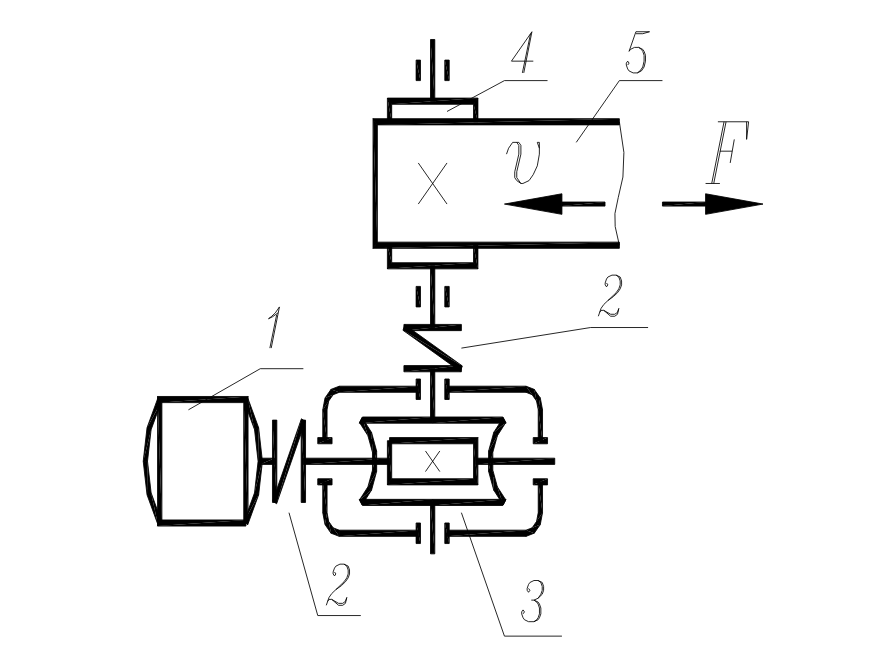
\includegraphics[width=0.7\linewidth]{方案}
		\caption[蜗轮蜗杆传动]{传动简图}
		\label{fig:}
	\end{figure}
	其中 1:电动机, 2:弹性联轴器, 3:蜗杆减速器, 4:滚筒, 5:带式运输机\ \
	\section{原动机选择}
	\subsection{电动机的选择}
	\begin{enumerate}
		\item[(1)] 按照工作要求,选择一般用途的\ YE3\ 系列超高功率三相异步电动机,电压380V
		\item[(2)] 选择电动机功率
		工作机所需效率为:
		$$P_w=\dfrac{F\cdot v}{1000}=\dfrac{\Ff \cdot \Vv}{1000}=\two{\Pw}\ kW$$
		传动装置总效率为:
		$$\eta	=\eta_\text{滚筒} \cdot \eta_\text{联轴器} \cdot \eta_\text{球轴承} \cdot \eta_\text{蜗轮蜗杆}
		=\ETAgt^\NUMgt\cdot \ETAgzzc^\NUMgzzc\cdot \ETAlzq^\NUMlzq\cdot \ETAwlwg
		=\two{\ETA}$$
		所需电动机功率为:
		
		$$P_d=\frac{P_w}{\eta}=\two{\Pd}\ kW \ \ \Longrightarrow P_{ed}=3 \ kW$$
		因为载荷平稳,电动机额定功率$P_{ed}$略大于$P_d$即可,查表后,选择电动机的额定功率$P_{ed}$为$\Ped\ kW$.
		\item[(3)] 确定电动机转速	滚筒轴的工作转速为
		$$n_w=\frac{60\cdot 1000\cdot \Vv}{\pi \cdot \Dd}=\two{\Nw}\ m/s$$
		一级蜗轮蜗杆减速器的传动比通常为$10\sim 20$,即$i_{a^{'}}=10\sim20$,故电动机转速可选范围为:
		$$n_{d^{'}}=i_{a^{'}}\cdot n_w=(\Nmin \sim \Nmax)\cdot n_w=\two{\Ndmin} \sim \two{\Ndmax} \ m/s$$
		符合这一范围的同步转速有$750r/min$,$1000r/min$,$\text{查阅相关标准}^{\cite{电动机}}$,根据功率,转速,挑选出以下两种型号电机,并进行比较.\par
		\begin{table}[h]
			\begin{tabular}{c|c|c|c|c|c|c}
				\hline
				方案 & 电动机型号 & 额定功率 /kW & 同步转速/满载转速$n_m$ & 重量   & 噪声   & 效率   \\
				\hline
				1    & YE3-132S-6 & \Ped         & 1000/960(/ r/min)      & 63$kg$ & 69$dB$ & 85.6\% \\
				\hline
				2    & YE3-132M-8 & \Ped         & 750/730(/ r/min)       & 61$kg$ & 64$dB$ & 82.5\% \\
				\hline
			\end{tabular} \ \
			\caption{电动机型号比较表}
		\end{table}
		
		
		为了使传动装置结构紧凑稳固,噪声更小,效率更高,选择方案1,确定电机型号为YE3-132S-6,
		其主要参数:满载转速$n_m=\Nm\ r/min,$中心高$H=132\ mm$,轴伸部分$D=38\ mm$
	\end{enumerate}
	\subsection{传动比的分配}
	总传动比:$i_a= \frac{n_m}{n_w}=\frac{960}{\two{\Nw}}=$%\two{\Ia}$,
	各个轴的传动比:$i_{01}=1$,$i_{12}=\two{\Ia}$
	\subsection{传动系统运动与动力参数计算}
	\newcommand{\T}[2]{\fpeval{9550* #1 / #2}}		%转矩计算函数
	\newcommand{\TL}{\T{\Pd}{\Nm}}					%T0电动机输出功率			
	\newcommand{\PI}{\fpeval{\Pd*\ETAI}}
	\newcommand{\PIO}{\fpeval{\PI*0.99}}			%设蜗杆轴效率为0.99			
	\newcommand{\NI}{\Nm}							%i01为1,此处不再定义
	\newcommand{\TI}{\T{\PI}{\NI}}					%N1=N0=Nm
	\newcommand{\TIO}{\fpeval{\TI*0.99}}
	\newcommand{\PII}{\fpeval{\PI*\ETAII}}
	\newcommand{\PIIO}{\fpeval{\PII*0.96}}			%设蜗轮轴效率为0.96
	\newcommand{\NII}{\fpeval{\NI / \Ia}}
	\newcommand{\TII}{\T{\PII}{\NII}}
	\newcommand{\TIIO}{\fpeval{\TII*0.96}}
	0轴(电动机轴)
	$$p_0=p_d=\two{\Pd}\  kW$$
	$$n_0=n_m=\Nm \  r/min$$
	$$T_0=9550 \frac{P_0}{n_0}=9550\times\frac{\two{\Pd}}{\Nm}=\two{\TL}  N\cdot m$$
	1轴(蜗杆轴)
	$$p_1=p_0 \eta_1=\Pd \times \ETAI=\two{\PI}\  kW$$
	$$n_1=\frac{n_0}{i_{01}}=\frac{\Nm}{1}=\Nm\  r/min$$
	$$T_1=9550 \frac{P_1}{n_1}=9550\times\frac{\two{\PI}}{\NI}=\two{\TI}\  N\cdot m$$
	\ \
	2轴(蜗轮轴)
	$$p_2=p_1 \eta_2=\two{\PI} \times \ETAII=\two{\PII}\  kW$$
	$$n_2=\frac{n_0}{i_{12}}=\frac{\Nm}{\two{\Ia}}=\two{\NII}\  r/min$$
	$$T_2=9550 \frac{P_2}{n_2}=9550\times\frac{\two{\PII}}{\two{\NII}}=\two{\TII}\  N\cdot m$$	\ \
	%	3轴(滚筒轴)
	%	$$p_3=p_2 \eta_3=2.361\times0.99^2=2.315\  kW$$
	%	$$n_3=\frac{n_2}{i_{23}}=\frac{50.259}{1}=50.259\  r/min$$
	%	$$T_3=9550 \frac{P_3}{n_3}=9550\times\frac{2.315}{50.259}=439.886\  N\cdot m$$ 
	根据以上计算结果,列出 各轴运动和动力参数 表如下:
	\begin{table}[h]  %动力参数表格
		\begin{tabular}{c|c|c|c|c|c|c|c} %表格位置: h:放在此处	t:放在顶端	b:放在底端	p:在本页 htbp:优先放在此处,其次是顶端,再次是底端.
			\hline
			\multirow{2}{*}{轴名} & \multicolumn{2}{c|}{功率\ $P/kW$}
			& \multicolumn{2}{c|}{转矩\ $T/N \cdot m$} & 转速        & 传动比     & 效率                                                 \\ \cline{2-5}
			& 输入                                     & 输出        & 输入       & 输出        & $n/(r/min)$ & $i$       & $\eta$       \\ \hline
			电动机轴              & \Ped                                     & \two{\Pd}   &            & \two{\TL}   & \Nm         &           &              \\
			1轴                   & \two{\PI}                                & \two{\PIO}  & \two{\TI}  & \two{\TIO}  & \NI         & 1         & \two{\ETAI}  \\
			2轴                   & \two{\PII}                               & \two{\PIIO} & \two{\TII} & \two{\TIIO} & \two{\NII}  & \two{\Ia} & \two{\ETAII} \\
			%滚筒轴  & 2.315  & 2.292   & 139.886 & 138.487 & 50.259      & 1      & 0.98   \\ 
			\hline
		\end{tabular}
		\caption{各轴动力参数表}
	\end{table}
	%-----------------欢呼吧!!第一部分编程结束了2021-6-21_03:06------------------------------
	%----------这一部分手选太多,自己查表修改,不在编程-----------------
	\chapter{传动零件的设计计算计}
	根据第一章计算的数据:电动机功率$P_{ed}=\Ped \ kW,$转速$n_1=\NI \ r/min$,传动比$i_{12}=\two{\Ia}$,载荷平稳单向回转.
	\section{传动类型选择} \ \
	根据$GB/T 10085-1998$\ \ 为了加工简便,易于更换维修,选择常用的右旋渐开线蜗杆(ZI蜗杆),精度等级为7级.
	\section{材料选择}
	根据工作要求,蜗杆选择45号钢,表面淬火处理,硬度达到45 $\sim$ 55 SRC, 蜗轮选择含锡量较低的5-5-5\ ZCuSn5Pb5Zn5的锡青铜金属模制造,轮芯采用灰铸铁HT100制造,
	\section{参数选择与强度计算}
	\subsection{传动比计算}
	在较大的传动功率下,为了提高效率,采用多头蜗杆,取$Z_1=2$,取传动比为19,则误差为$\Delta=\frac{19.101-19}{19.101}\times100\%=0.53\%$,在误差允许范围内.再根据效率传动比与蜗杆头数,蜗轮齿数的关系:$i_{12}=\frac{n_1}{n_2}=\frac{Z_2}{Z_1}$,计算得到:$Z_2=Z_1 \cdot i_{12}=2\cdot19=38$,查表12-8,估计$\eta=0.8$
	
	\subsection{强度计算}
	因为圆柱蜗杆传动的主要失效形式为蜗轮轮齿表面产生胶合,点蚀,磨损,所以根据蜗轮齿面疲劳接触强度进行设计计算.\ \
	已知蜗轮所受的的转矩$T_2=\three{\TII}$,因为工作转速不大,工作冲击不大,环境温度不高,故选择使用系数{\color{red}$\ K_A=1.20$.}因为蜗杆采用45号钢,其硬度大于45SRC,蜗轮选择ZCuSn5Pb5Zn5的锡青铜金属模制造,单向旋转,根据表12-2选取综合弹性系数${\color{red}Z_e=160\ }$,查表12-4,许用接触应力${\color{red}[\sigma_H ]=220Mpa}$,查表12-6,许用弯曲用力${\color{red}\ [ \sigma_F ]=28Mpa}$.
	$Z_p$为接触系数,先假设蜗杆分度圆直径$d_1$和中心矩$a$的比值$\frac{d_1}{a}=0.37$,查表得到${\color{red}Z_p=2.8}$.\ \
	
	根据赫兹公式,得到蜗轮齿面疲劳接触强度的设计公式如下$$a\ge\sqrt[3]{K_AT \Bigl(\frac{Z_e Z_p}{[ \sigma_H ]} \Bigl)^2} $$
	所以中心矩为:
	$$a\ge\sqrt[3]{1.20\times 447284.28\times10^3 \Bigl(\frac{160\times2.8}{220} \Bigl)^2}= 131.597\ mm$$
	\subsection{参数确定}
	\paragraph{1.参数的估算与选择}
	$$d_1\approx 0.68a^{0.875}=0.68\times130.565^{0.875}=48.62\ mm$$
	$$m\approx \frac{2a-d_1}{Z_2}=\frac{2\times130.565-48.290}{38}=5.646\ mm$$
	$$a=0.5m(q+Z_2)=0.5\times6.3(10+38)=151.2\ mm>131.597 \ mm$$\par
	查表12-1选择$m=6.3\ mm,\ d_1=63\ mm,\ q=10.00,\ d_2=mZ_2=6.3\cdot38=239.4\ mm$
	因为$a=151.2\ mm>131.597\ mm$	故接触强度足够.由蜗轮传动中心矩的标准系列(...,80,100,125,160,180,...),选取中心矩$a=160\ mm$,但如果选取此值,则会引起传动比变化,而且对于模数$m=6.3$而言,不存在任何整数齿数使得$a=160$,在改变传动比的情况下,要圆整中心矩会导致工作机转速达不到要求,在不改变传动比的情况下要圆整,需要在滚切蜗杆时将滚刀相对于蜗轮中心向外移动8.8mm,假设这样做引起的变位系数在正常范围内,那么就采取变位传动方式.
	\paragraph{2.最终参数} 根据以上计算结果,蜗杆的具体参数如下表所示:
	
	%------------------------Note---------------------
	%此处可以编程
	%-------------------------------------------------
	
	
	\begin{table}[h]\centering
		\begin{tabular}{cc}
			\hline
			\multicolumn{2}{c}{蜗杆参数}                                                                        \\ \hline
			\multicolumn{1}{c|}{分度圆直径}   & $d_1=mq=6.3\cdot10=63\ mm$                                      \\ \hline
			\multicolumn{1}{c|}{分度圆导程角} & $\gamma=arctan\frac{Z_1}{q}=arctan(\frac{2}{10})=11.31^{\circ}$ \\ \hline
			\multicolumn{1}{c|}{齿顶高}       & $h_a=m=6.3\ mm$                                                 \\ \hline
			\multicolumn{1}{c|}{齿根高}       & $h_f=1.2m=1.2\cdot6.3=7.56\ mm$                                 \\ \hline
			\multicolumn{1}{c|}{齿顶圆直径}   & $d_{a1}=m(q+2)=6.3\cdot(10+2)=75.6\ mm$                         \\ \hline
			\multicolumn{1}{c|}{齿根圆直径}   & $d_{f1}=m(q-2.4)=6.3\cdot(10-2.4)=47.88\ mm$                    \\ \hline
			\multicolumn{1}{c|}{轴向齿距}     & $P_a=\pi m=19.792\ mm$                                          \\ \hline
			\multicolumn{1}{c|}{轴向齿厚}     & $S_a=\frac{1}{2}\pi m =9.896\ mm$                               \\ \hline
			\multicolumn{1}{c|}{法向齿厚}     & $S_n=S_a\cdot \cos\gamma=9.704\ mm$                             \\ \hline
		\end{tabular}
		\caption{蜗杆轮齿参数表}
	\end{table}\newpage
	蜗轮的具体参数如下表所示:
	\begin{table}[h]\centering
		\begin{tabular}{cc}
			\hline
			\multicolumn{2}{c}{蜗轮参数}                                                      \\ \hline
			\multicolumn{1}{c|}{分度圆直径} & $d_2=mZ_2=6.3\cdot38=239.4\ mm$                 \\ \hline
			\multicolumn{1}{c|}{齿顶高}     & $h_a=m=6.3\ mm$                                 \\ \hline
			\multicolumn{1}{c|}{齿根高}     & $h_f=1.2m=1.2\cdot6.3=7.56\ mm$                 \\ \hline
			\multicolumn{1}{c|}{喉圆直径}   & $d_{a2}=m(Z_2+2)=6.3\cdot(38+2)=252\ mm$        \\ \hline
			\multicolumn{1}{c|}{齿顶圆直径} & $d_{e2}\le d_{a2}+1.5m=261.45\ mm$              \\ \hline
			\multicolumn{1}{c|}{齿根圆直径} & $d_{f2}=m(Z_2-2.4)=6.3\cdot(38-2.4)=224.28\ mm$ \\ \hline
			\multicolumn{1}{l|}{轮缘宽度}   & $B\le 0.75d_{a1}=0.75\cdot 75.6=56.7\ mm$       \\ \hline
			\multicolumn{1}{l|}{轮圈宽度}   & $C=1.65m+1.5=10.389+1.5=11.895\ mm$             \\ \hline
		\end{tabular}
		\caption{蜗轮参数表}
	\end{table}\ \
	\section{参数校核}
	\subsection{强度校核}
	根据以上的最终参数,按齿根弯曲强度进行校核,校核公式如下:
	$$\sigma_F=\frac{1.53K_AT_2Y_{Fa2}}{d_1d_2m\cos\lambda}\le[\sigma_F]$$
	当量齿数:\ \ $Z_{Y2}=\frac{Z_2}{\cos^3\lambda}=\frac{38}{\cos^311.31^\circ}=40.303\approx41$\ \
	齿形系数:根据$Z_{Y2}=41$,从图11-9中可以查得齿形系数\ \ {\color{red}$Y_{Fa}=2.45$}\ \
	螺旋角系数:\ \ $Y_\beta=1-\frac{\sigma}{140^{\circ}}=1-\frac{11.31^{\circ}}{140^{\circ}}=0.9192$
	之前查表得:许用弯曲用力${\color{red}\ [ \sigma_F ]=30Mpa}$
	蜗轮齿根弯曲应力:
	$$\sigma_F=\frac{1.53K_AT_2Y_{Fa2}}{d_1d_2m\cos\lambda}=\frac{1.53\times 1.2 \times 457983\times 2.45}{63\times 239.4 \times 6.3 \times \cos11.31^{\circ}}=22.11 \ Mpa <[\sigma_F]=28\ Mpa$$
	满足弯曲强度.\ \
	对$Z_p$校核:$\frac{d_1}{a}=\frac{63}{160}=0.394$,查表可得$z_{p'}=2.75<2.9$,故以上计算过程有效.
	\subsection{传动效率校核}
	%寿命系数\ \ $K_{PN}=\sqrt[9]{\frac{10^6}{3.181}}$
	蜗杆转速:$V_1=\pi n\frac{D_1}{60\cdot 1000}=3.12\ m/s$\ \
	蜗轮转速:$V_2=\frac{V_1}{\cos(\gamma)}=3.23 \ m/s$\ \
	传动效率:
	$$\eta=\frac{tan\lambda}{tan(\lambda+\rho^{'})}=\frac{tan11.31^{\circ}}{tan(11.31^{\circ}+1.37^{\circ})}=0.88>0.84$$
	%效率贼高,许用应力贼大,贼安全,贼有前瞻性的设计.^_^(巨浪费...)#6-21已经修改,不再过分安全了
	效率大于之前的估计值,可以使用.\ \
	\subsection{热平衡计算}
	\paragraph{1.估算散热面积$A$}
	\newcommand{\Aafinal}{\fpeval{0.33*(\Aa/100)^1.75}}
	$A=0.33\cdot \Bigl( \frac{\Aa}{100} \Bigl) ^{1.75}=\two{\Aafinal}\ m^2$
	\paragraph{2.验算油的工作温度$ti$}
	室温下$t_0=20\circ$,散热系数$:\alpha_t=13\ W/(m^2\cdot \ ^{\circ}C) $可以计算$\Delta t$:
	$$\Delta t=\frac{1000(1-\eta)P_1}{\alpha_tA}
	=\frac{1000(1-\two{\ETAII})\cdot \two{\PI}}{\alpha_tA}
	=47.1<60\ ^{\circ}C$$
	所以$t_{max}=20+47.1=67.1<90,$没有超过温度允许值,故不需要采取冷却措施.
	

	
	\chapter{主要零部件设计}
	\section{轴的设计}
	\subsection{蜗杆的结构设计}
	
	%**************重要数据定义********************
	\newcommand{\C}{110}
	%----------------计算结果------------->>>>>>>>>
	\newcommand{\DminI}{\fpeval{\C*(\PI/\NI)^(1/3)}}
	\newcommand{\DminII}{\fpeval{\C * (\PII/\NII)^(1/3) }}
	\newcommand{\DminIp}{\fpeval{\DminI*1.03}}
	
	
	\paragraph{1.方案确定} 一级蜗轮蜗杆减速器可以将蜗杆安排在箱体中间,两侧滚动轴承成对分布,轴承用轴肩定位,一段固定,一端游离,联轴器用平键连接定位.\ \
	蜗杆上的参数:{\color{red}	功率$P_1=\two{\Pd}\ kW$,	转速$N_1=\Nm\ r/min$,转矩$T_1=\two{\TI}\ N\cdot m$}
	\paragraph{2.按纯扭转初步估算最小轴径}
	由于轴选择的是45号钢,查表14-2得$\ [t]=30\sim40,\ C=117\sim107$,这里选取$C=110$,对于只受转矩的轴而言,其设计公式为:
	$$ d\ge C\sqrt[3]{\frac{P}{n}}=110\cdot \sqrt[3]{\frac{3.181}{960}}=\two{\DminI}\ mm$$
	由于轴上含有键槽,故增大$3\%$的直径:$d=\two{\DminI} \cdot103\%=\two{\DminIp}\ mm\Longrightarrow d=20.00\ mm$
	\paragraph{3.轴上各段参数的确定}
	\begin{enumerate}
		\item[(1)] I端(联轴器端)\ \
		\newcommand{\Zhou}[4]{$|d_#1=#2$\par$|L_#3=#4$}
		\marginpar{\footnotesize {\color{blue}\Zhou{1}{32}{1}{88}}}
		联轴器的选取:根据所受转矩$T_1=\two{\TI}\ N\cdot m$,则联轴器所受转矩为:
		$T_{ca}=K_A T_1=1.3\times \two{\TI}=37.11\ N\cdot m$,根据电动机输入轴参数,与公称直径的要求,查表6-96($P_{146}$)选取弹性套柱销联轴器LT5$\ \frac{ZC44\times28}{32\times82}$GB/T\ 4323-2017,考虑到联轴器的安装尺寸,所以这里取$d_1=32\ mm,L_1=82+6=88\ mm$\par
		键的选择:根据轴的公称直径,查表$6-54(P_{111})$,选取A型平键,剖面尺寸为:$10\times8$,键长$l$取88-8=80\ mm,
		即GB/T\ 1096\ $10\times8$
		
		\item[(2)] II端(左侧轴承端盖端)\ \
		\marginpar{\footnotesize {\color{blue}\Zhou{2}{42}{2}{50}}}
		因为定位键高度$h=10\ mm$查表得嵌入到轴的深度为5,则伸出的高度为:5\ mm,$d_2=d_1+2h=42\ mm$,选取凸缘式轴承盖,其总长为$20\ mm$,取轴承端盖外端面与联轴器内端面距离为$L=30\ mm$,所以$L_2=30+20=50\ mm$
		
		\item[(3)] III端(轴承端)\ \
		\marginpar{\footnotesize {\color{blue}$|d_3=45$\par  $|L_3=22$\par $|L_{3^{'}}=25$}}
		根据此轴的受力与轴的公称直径,查表6-64$P_{126}$,暂选圆锥滚子轴承,根据要求选取$30208$ GB/T\ 297-2015,
		其参数为:$d\times D \times B=45\times 85 \times 20.75$长度取$L_3=16+6=22\ mm.$进而可以确定,其用于定位的套筒直径为50(<53),轴肩的直径为53(>52),
		
		\item[(4)] IV端(轴肩端)\ \
		\marginpar{\footnotesize {\color{blue}\Zhou{4}{53}{4}{10}}}
		起定位作用的轴肩,高度$d=d+(3\sim 4)C=45+2*4=53\ mm$,长度取$10\ mm$
		\item[(5)] V端(蜗杆端)\ \
		
		\marginpar{\footnotesize {\color{blue}$|d=63$\par $|d_{a1}=75.6$\par $|b_1=84$}}
		由之前的设计选取知道蜗杆的分度圆直径$d=63\ mm$,齿顶圆直径$d_{a1}=75.6\ mm$,蜗杆的喉圆直径$d_{a2}=252\ mm$.
		所以,蜗杆轴的长度$b_1=(11+0.06Z_2)m=(11+0.06\times 38)\cdot6.3=83.664\ mm$,圆整到85\ mm.
		\item[(6)] VI端(蜗杆旁置端)\ \
		\marginpar{\footnotesize {\color{blue}\Zhou{6}{58}{6}{25}}}
		为保证蜗杆与箱体之间有一定间隙,两侧各取$L_6=25\ mm$,直径取$d_6=d_3+5=48\ mm$
	\end{enumerate}
	%---------------------------------------------------------
	\subsection{蜗杆轴的校核}
	\paragraph{1.受力分析}
	
	\newcommand{\DI}{63}
	\newcommand{\DII}{239.4}
	\newcommand{\LI}{0.17}		%两轴承力作用点之间的距离(这里的设计是轴承关于齿轮中心对称分布)
	\newcommand{\KI}{0.107}		%联轴器端力作用点轴上投影到最近一端轴承力作用点之间的距离
	\newcommand{\FaII} {\fpeval{\TI*2/\DI*1000}}  %\FtII
	\newcommand{\FtII} {\fpeval{\TII*2/\DII*1000}}	%FaII
	\newcommand{\FrII}{\fpeval{\FtII*tand(20)}}	%FrI
	%	\newcommand{\FIV}{\fpeval{\FrII/2}}
	\newcommand{\FIH}{\fpeval{\FaII/2}}
	\begin{figure}[h]
		\centering
		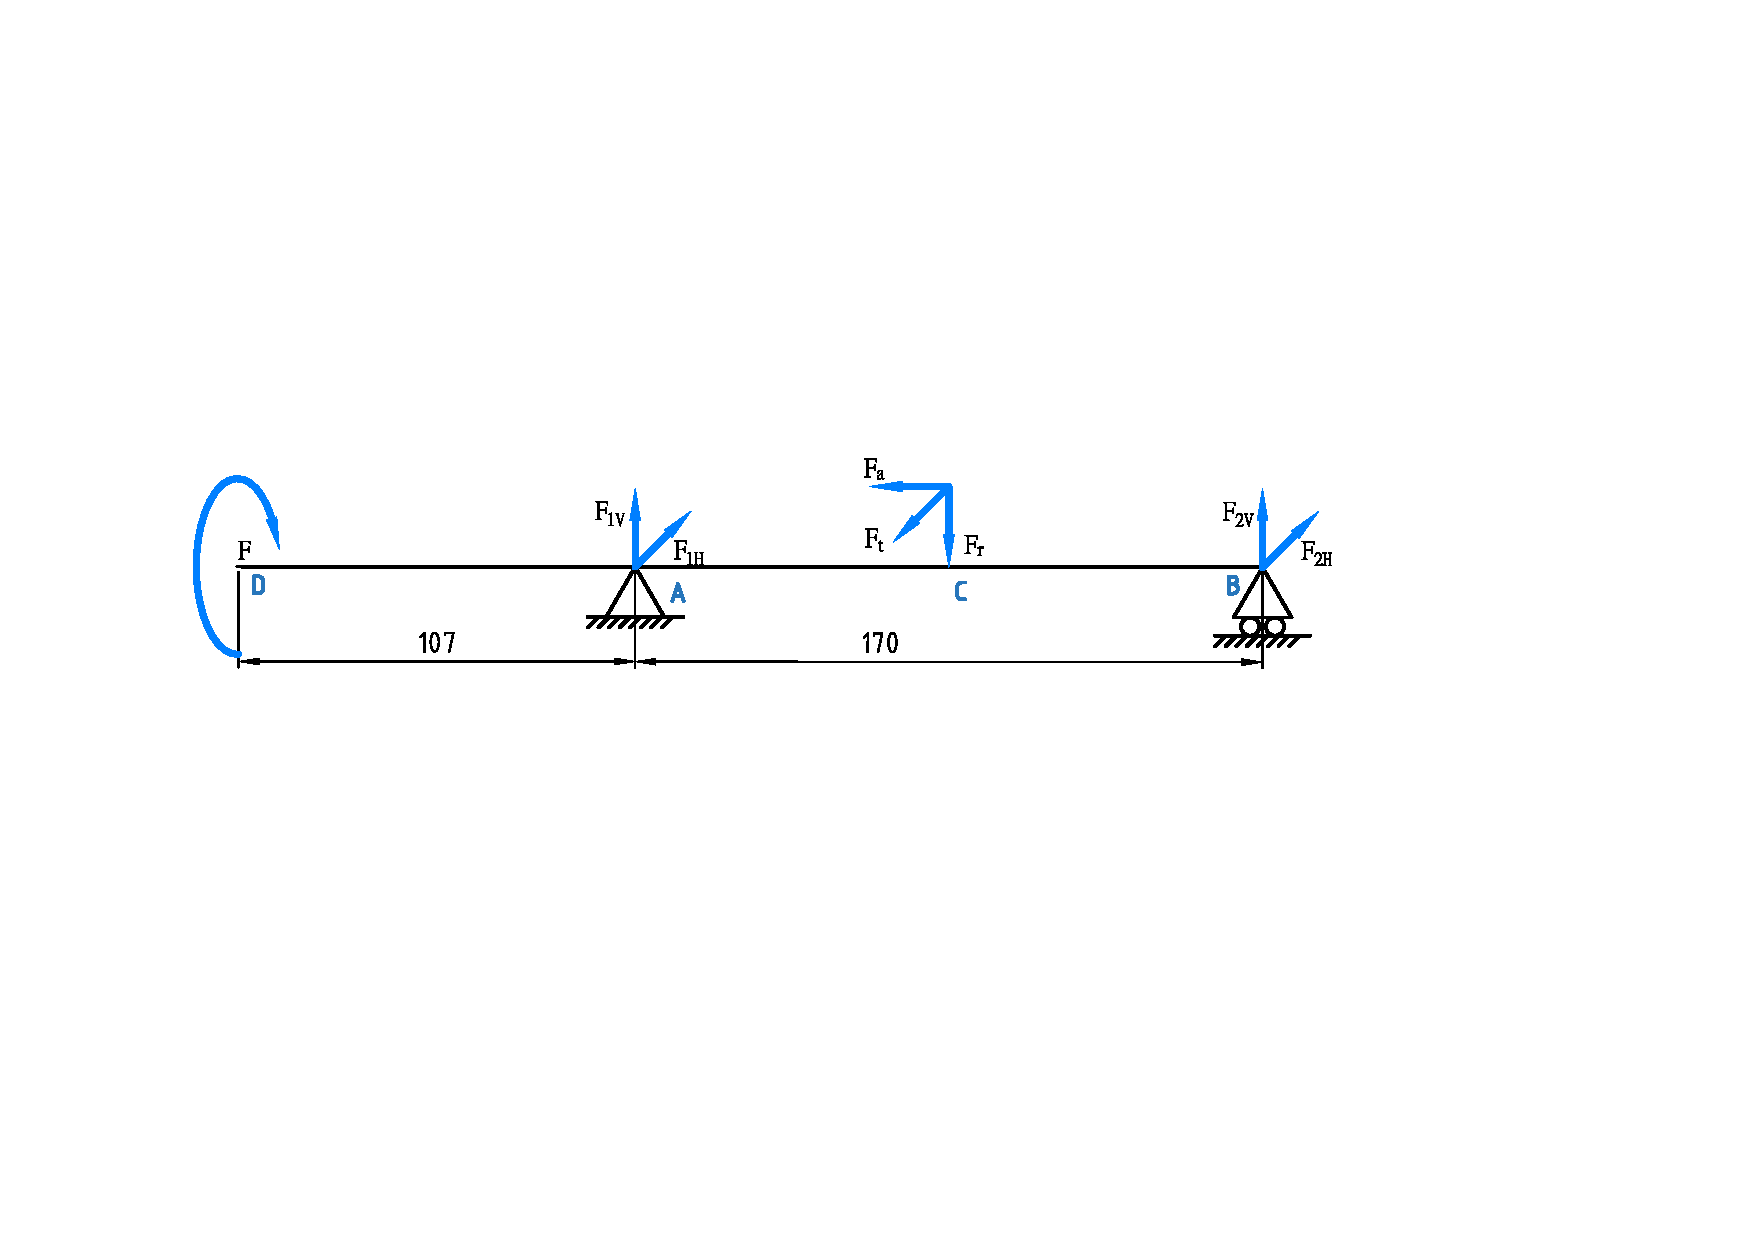
\includegraphics[width=1\linewidth]{蜗杆轴受力图}
		\caption[蜗杆轴]{蜗杆轴受力图}
	\end{figure}
	已知蜗杆的分度圆直径为$d_1=63\ mm.L_1=170\ mm,K_1=107$
	经受力分析可得%${\text{\emoji{point-down}}}$
	$$	\begin{cases}
		$$\text{切向力:}F_{t1}=F_{a2}=\frac{2T1}{d1}=\frac{2\times \two{\TI}}{\DI}\cdot1000= \two{\FaII} \ N$$   \\
		$$\text{径向力:}F_{r1}=F_{r2}=F_{t2}\cdot \tan{\alpha} =\two{\FtII}\cdot
		0.369=\two{\FrII}\ N$$                                                                                   \\
		$$\text{轴向力:}F_{a1}=F_{t2}=\frac{2T_2}{d_2}=\frac{2\times \two{\TII}}{\DII}\cdot1000=\two{\FtII}\ N$$ \\
		%$$\text{左转矩:} M_1=T_1=31664\ N\cdot mm $$ \text{\ \ \footnotesize (方向未确定)}
	\end{cases}$$
	%---------------------------------------------------------------------////////////---------
	\newcommand{\MaI}{103.511}
	\newcommand{\FIV}{\fpeval{(\FrII*\LI/2-\MaI)/\LI}}
	\newcommand{\FIIV}{\fpeval{(\FrII*\LI/2+\MaI)/\LI}}
	\newcommand{\MVmax}{\fpeval{\FIIV*\LI/2}}
	\newcommand{\MHmax}{\fpeval{\FIH*\LI/2}}
	%\newcommand{\Mmax}{\fpeval{\Mvmax+\MHmax+\TI}}
	由于切向力力$F_t$只产生弯矩,在铅垂平面上,力$F_{a1}$产生弯矩$M_{a1}=F_{a1}\times \frac{d_1}{2}=\two{\MaI}\ N\cdot m,$分析受力,分别对A\dunhao B点取矩,可得:%$\displaystyle \sum_{i=1}^{n} M_i=0$
	$$\begin{cases}
		F_{1V}=\frac{F_{r1}\cdot \frac{L_1}{2}+M_{a1}}{L_1}=\two{\FIIV}\ N \\
		F_{2V}=\frac{F_{r1}\cdot \frac{L_1}{2}-M_{a1}}{L_1}=\two{\FIV}\ N
	\end{cases}$$
	%\ \ 解之得:$F_{1V}=F_{2V}=\two{\FIV}\ N$\ \ 
	所以铅垂面上最大扭矩为:$M_{Vmax}=F_{1V}\cdot \frac{L_1}{2}=\two{\MVmax}\ N\cdot m$\par
	在水平面上,由平面力系平衡方程可得水平面的支撑反力:
	$$\begin{cases}
		F_{1H}=\frac{F_{t1}\cdot\frac{L_1}{2}}{L_1}=\two{\FIH}\ N \\%\text{\emoji{zero}}\\
		F_{1H}=\frac{F_{t1}\cdot\frac{L_1}{2}}{L_1}=\two{\FIH}\ N
	\end{cases}$$
	%解之得:$F_{1H}=F_{2H}=\two{\FIH}\ N$\\
	所以水平面上最大扭矩为:$M_{Hmax}=F_{1H}\times \frac{L_1}{2}=\two{\MHmax\ N\cdot m}$\par
	左侧的转矩为:$M_1=\two{\TI}$,所以危险截面C的扭矩为:$M_{max}=M_{Hmax}+M_{Vmax}+M_1=177.99\ N\cdot m$
	\paragraph{2.扭矩图}
	经过以上计算可以画出蜗杆轴的扭矩图如下:\newpage
	\begin{figure}[h]
		
		\centering
		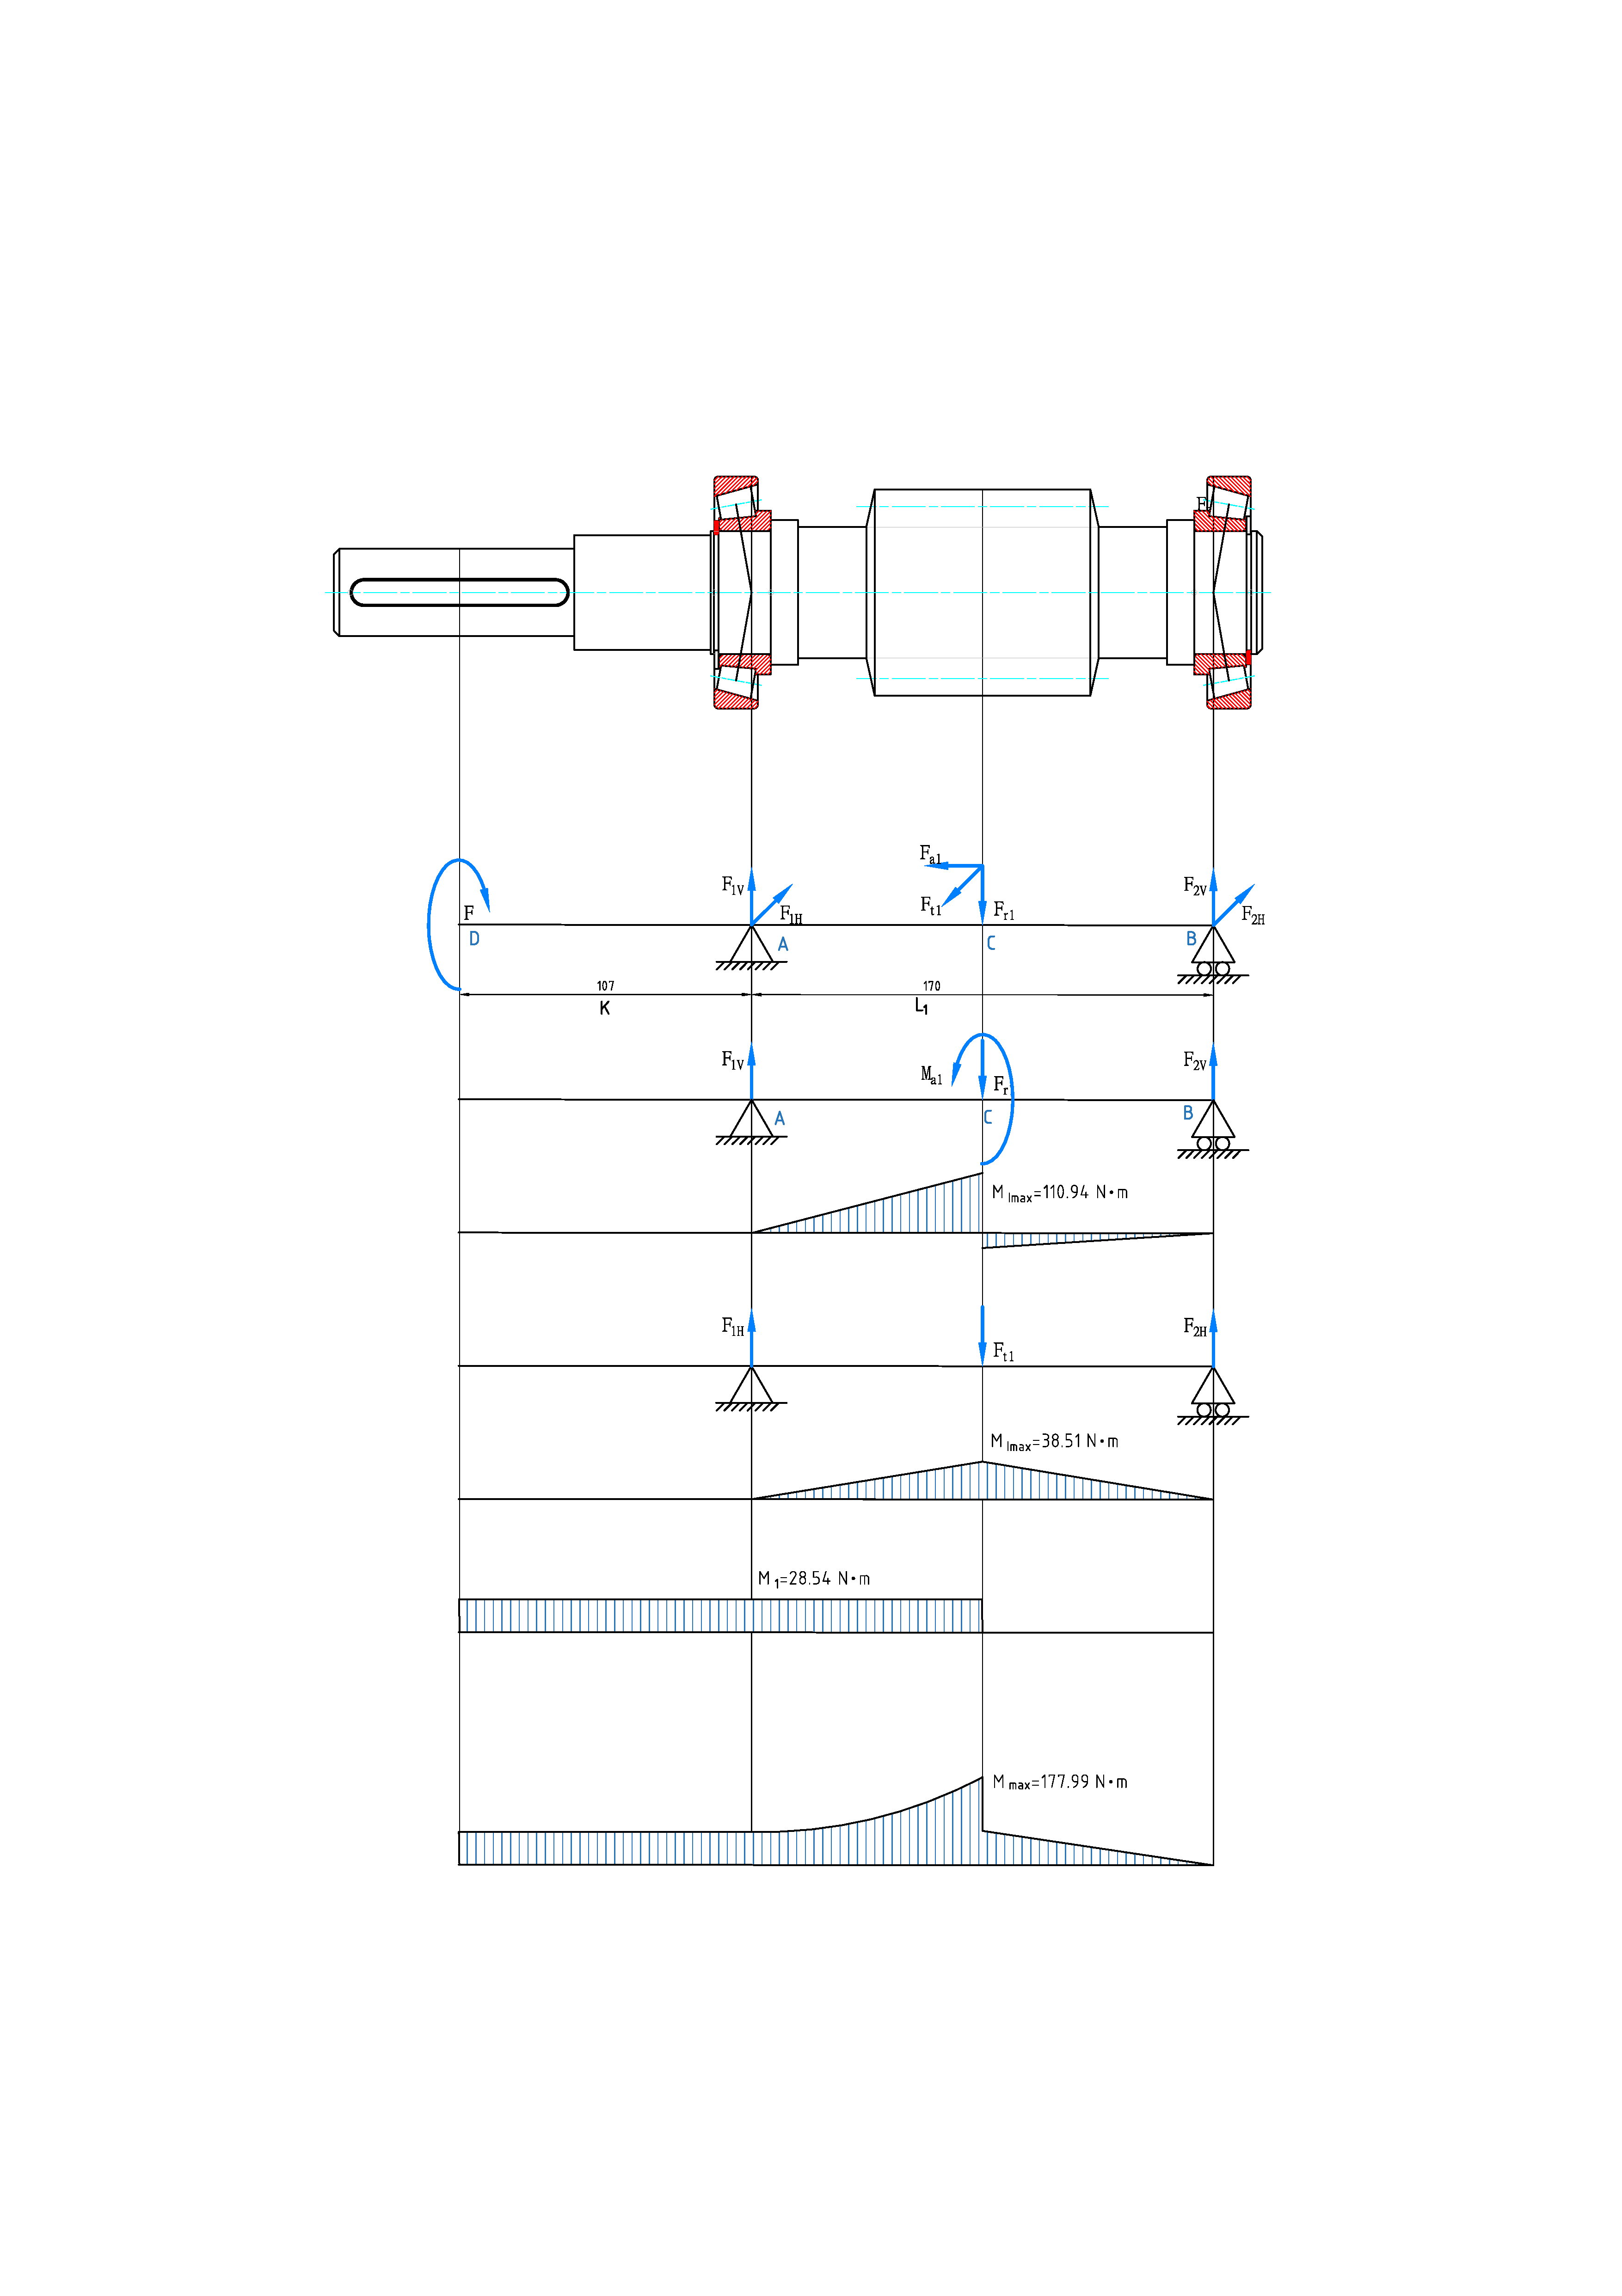
\includegraphics[width=0.9\linewidth]{蜗杆轴扭矩图}
		\caption{蜗杆轴扭矩图}
	\end{figure}
	
	\paragraph{3.危险截面强度校核}
	C截面的应力$\sigma_C=\frac{M_{max}}{0.1\cdot {d_1}^3}=7.11<[\sigma_F]=28\ Mpa$
	\paragraph{4.联轴器强度校核}
	此联轴器参数为:LT5$\ \frac{ZC44\times28}{32\times82}$GB/T\ 4323-2017,
	其\textbf{公称转矩为}:$T_n=224 \ N\cdot m \ge T_{ca}=K_A T_1=1.3\times \two{\TI}=37.11\ N\cdot m$,满足要求。
	\paragraph{5.轴上零件的定位与连接方式}
	\begin{enumerate}
		\item[(1)] 联轴器与轴采用A型平键定位连接%(两头是半圆)
		连接,参数为:GB/T\ 1096\  \ 键\ \ 20$\times$70,采用完全对称偏差配合.\ \
		\item[(2)]轴承端盖通过轴承套筒定位,不与轴连接.
		\item[(3)]套筒通过凸台,轴肩定位,与轴采用间隙配合$\frac{H7}{h6}$   %都是基轴制
		\item[(4)]滚动轴承用轴肩定位,采用过盈配合$\frac{P7}{h6}$,
	\end{enumerate}
	\paragraph{6.蜗杆轴(高速轴)键的校核}
	设载荷为均匀分布,可以计算得到该平键的挤压强度条件:
	\newcommand{\SiI}{\fpeval{40*\TI /(20*12*70*0.01)}}
	$$\sigma_p=\frac{4T}{dhl}=\frac{4\cdot \two{\TI}\cdot 10^{2}}{20\cdot 12 \cdot 70}= \two{\SiI}\le [\sigma_p]=60\ MPa$$
	选取45钢作为轮毂的材料,由以上计算可知,键的选取满足要求。
	\paragraph{7.轴承的校核}
	轴承选取$30208$ GB/T\ 297-2015,其参数为:$d\times D \times B=45\times 85 \times 20.75$长度为$L_3=16+6=22\ mm$,其额定动载荷为$C_r=63000\ N$极限转速为5000,寿命取$10000h$	由受力分析易得左端为压紧端,查表可得$f_t\text{(温度系数)}=1,f_p\text{(载荷系数)}=1.2,\epsilon=\frac{3}{10}$由公式
	\begin{align*}
		C_r &= \frac{f_pP}{f_t}(\frac{60n}{10^6}L_h)^{\frac{1}{\epsilon}} \\
	  63000 &= \frac{1.2\times P}{1}(\frac{60\times 960}{10^6}\times 10^4)^{\frac{3}{10}} \\
		  P=F_r &= \frac{52500}{576^{0.3}}=7798> \two{\FrII}\ N
	\end{align*}
	所以轴承满足要求。
	
	%---------------------------------------------------------
	
	\subsection{蜗轮轴的结构设计}
	\paragraph{1.方案确定} 一级蜗轮蜗杆减速器可以将蜗轮安排在箱体中间,两侧滚动轴承成对分布,轴承用轴肩定位,一段固定,一端游离,分别从左右两侧装入蜗轮左面用轴肩定位,右面用轴端盖定位,轴向采用键和过渡配合,联轴器用平键连接定位.\\
	蜗轮轴的参数:{\color{red}	功率$P_2=\two{\PII}\ kW$,	转速$N_2=\two{\NII}\ r/min$,转矩$T_2=\two{\TII}\ N\cdot m$}
	\paragraph{2.按纯扭转初步估算轴径}
	计算轴上受力:\ \
	(1)蜗轮轴向力\ $F_{a2}=F_{t1}= \two{\FaII} \ N$\ \
	(2)蜗轮周向力\ $F_{t2}=F_{a1}= \two{\FtII}\ N$\ \
	(3)蜗轮径向力\ $F_{r2}=F_{r1}= \two{\FrII}\ N$\ \
	由于轴选择的是45号钢,查表14-2得$\ [t]=30\sim40,\ C=117\sim107$,这里选取$C=110$,对于只受转矩的轴而言,其设计公式为:
	$$ d\ge C\sqrt[3]{\frac{P_2}{n_2}}=\C\cdot \sqrt[3]{\frac{\two{\PII}}{\two{\NII}}}=\two{\DminII}\ mm$$
	由于轴上含有键槽,故增大$3\%$的直径:$d=\two{\DminII}\cdot103\%=41.16\ mm\Longrightarrow d=46\ mm$
	
	\paragraph{3.轴上各段参数的确定}
	\begin{enumerate}
		\item[(1)] I端(联轴器端)\ \
		\marginpar{\footnotesize {\color{blue}$|d_1=50$\par  $|L_1=84$\par  $|L=70$}}
		联轴器的选取:根据所受转矩$T_2=\two{\TII}\ N\cdot m$,则联轴器所受转矩为:
		$T_{ca}=K_A T_1=1.3\times \two{\TII}=595.37\ N\cdot m$,根据公称直径的要求,查表选取弹性套柱销联轴器LT8$\ \frac{50\times84}{60\times142}$GB/T\ 4323-2017(蜗轮轴为主动端,), 轴上键槽取$18\times10,L=70\ mm$.\ \
		%	------------------------------------------
		\item[(2)] II端(左侧轴承端盖端)\ \
		\marginpar{\footnotesize {\color{blue}$|d_2=62$\par  $|L_2=55$}}
		取定位销键高度$h=10\ mm$,轴肩高度$d_2=d_1+2\times6=\fpeval{50+2*6}\ mm$轴承端盖总长为$20\ mm$,取轴承端盖外端面与联轴器内端面距离为$L=20\ mm$,所以$L_2=35+20=55\ mm$ 	%有点随意!!!_随便是不行的,现在明白了吧,之前贼丑,到底还是要反过来验证,一步步才能找到合适的尺寸.
		\item[(3)] III端(轴承端)\ \
		\marginpar{\footnotesize {\color{blue}$|d_3=70$\par  $|L_3=50$}}
		根据此轴的受力情况,暂选圆锥滚子轴承,根据要求选取$30214$ GB/T\ 297-2015,
		其参数为:$d\times D \times B=70\times125\times22$考虑到角接触球轴承右端用套筒来向轴肩定位,
		轴承右端面距齿轮中心距离为$63\ mm$,轴承宽度$B=22\ mm$,左端伸出$2\ mm$,所以$d_{z1}=24-2=20\ mm$,
		凸台宽度$15\ mm$,套筒长度$11\ mm$,轮伸出$4\ mm$,所以轴承端$L_{3}=15+11+20+4=50\ mm$
		
		
		%取齿轮距离箱体$a=20\ mm$,考虑到箱体误差在确定滚动轴承时应距箱体内壁一段距离$S=8\ mm$,则$L_3=B+a+S=20+20+8=48\ mm\Longrightarrow 50\ mm.$
		\item[(4)] V端(蜗轮端)\ \
		\marginpar{\footnotesize {\color{blue}$|d_4=66$\par  $|L_4=66$}}
		为了安装蜗轮,选取$d_4=66\ mm$,蜗轮齿宽$L_{蜗轮}=0.75\cdot 75.6=56.7\ mm$,为了能压紧蜗轮,取$L_4=66\ mm$
		\marginpar{\footnotesize {\color{blue}$|d_5=90$\par  $|L_5=10$}}
		\item[(5)]  V轴肩端
		为了轴环的轴向定位,取$d_5=90\ mm$,$L_5=10\ mm$
		\marginpar{\footnotesize {\color{blue}$|d_6=70$\par  $|L_6=38$}}
		\item[(6)] 端盖端
		根据端盖的要求,选取$d_6=70\ mm$
		让两侧中心距一致,取凸台宽度$13$,轴承宽度$20$,端盖上$e=12,m=18,m-e1=5,,e_1=13(要求大于e),$所以$L_6=5+20+13=38\ mm$
	\end{enumerate}
	
	%---------------------------------------------------------
	\newpage
	\subsection{蜗轮轴的校核}
	\paragraph{1.受力分析}
	
	\begin{figure}[h!]
		\centering
		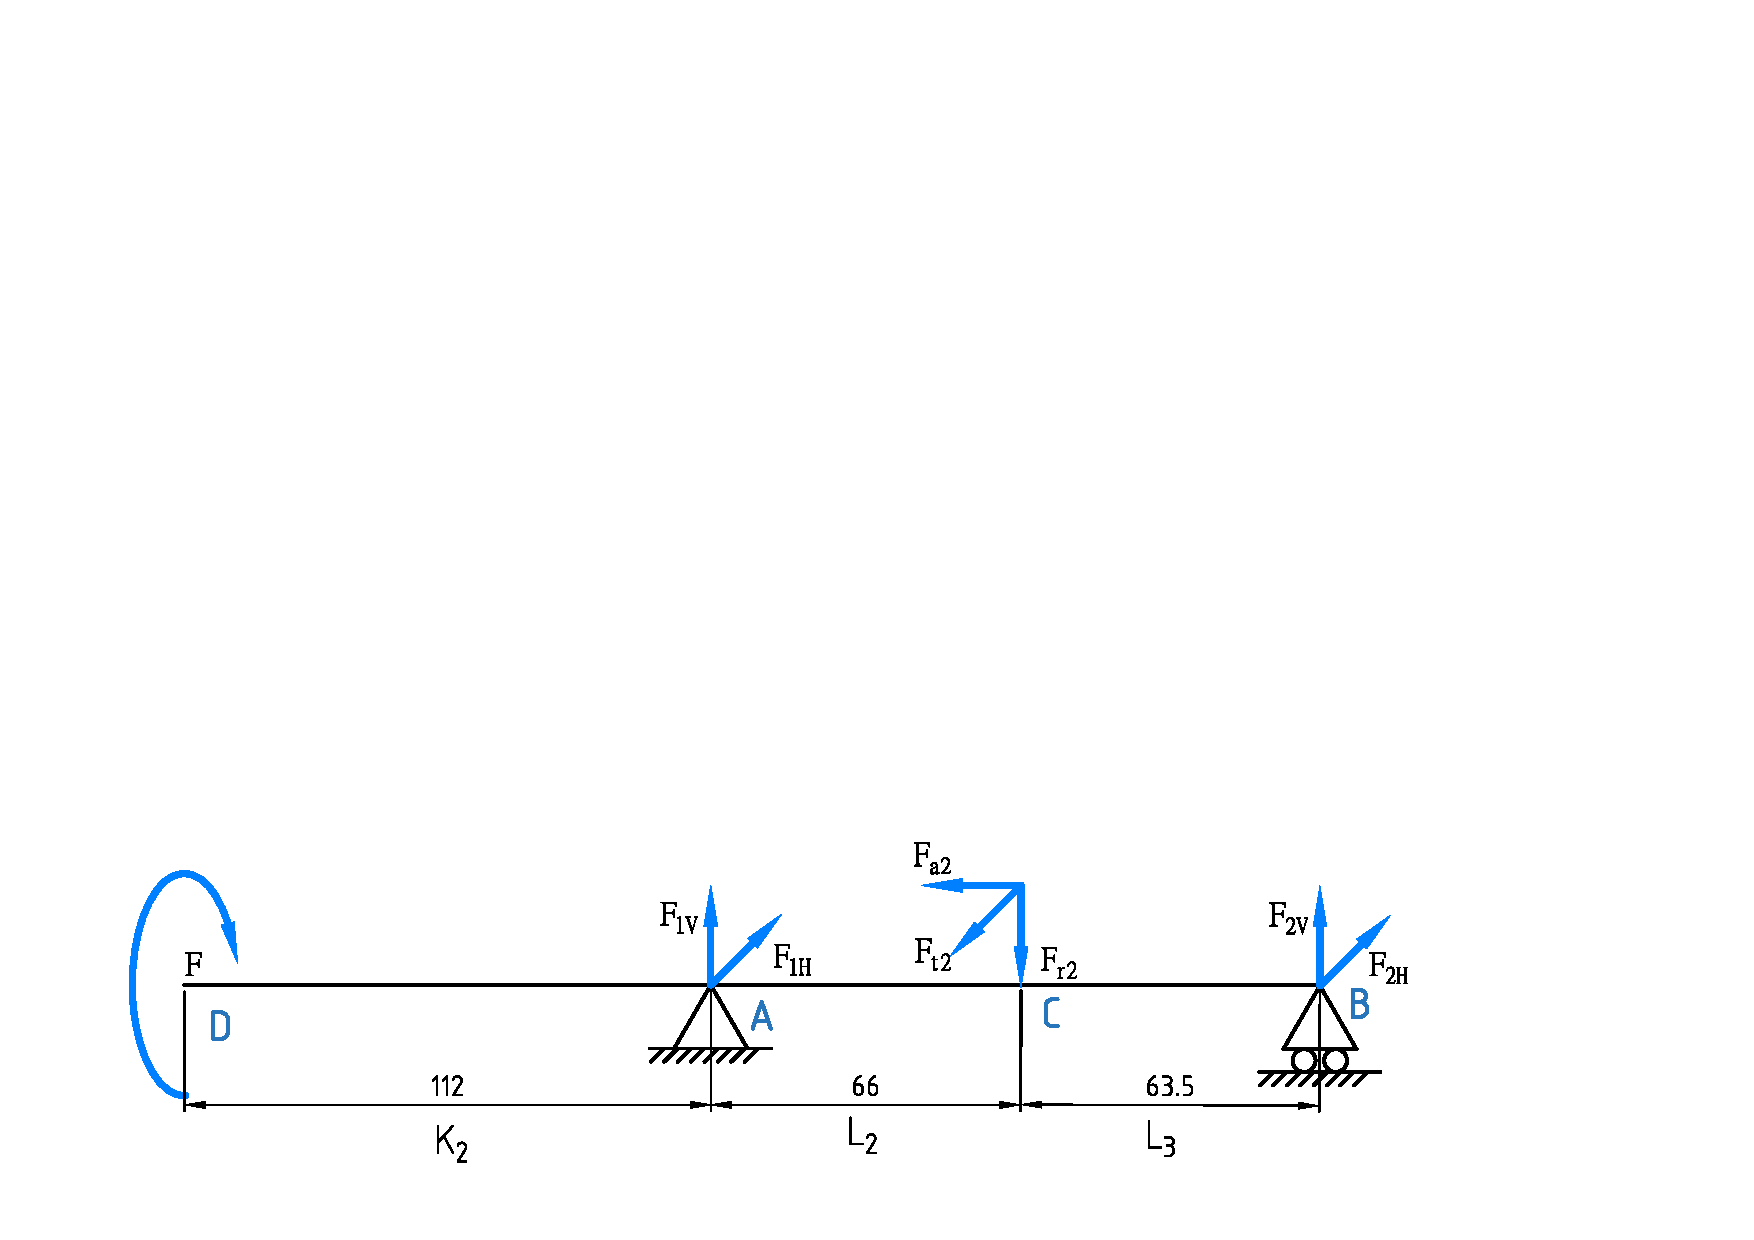
\includegraphics[width=1\linewidth]{蜗轮轴受力图}
		\caption[蜗轮轴]{蜗轮轴受力图}
	\end{figure}
	
	已知蜗轮的分度圆直径为$d_2=239.4\ mm.L_1=170\ mm,K_1=107$
	经受力分析可得%${\text{\emoji{point-down}}}$
	$$	\begin{cases}
		$$\text{切向力:}F_{a2}=F_{t1}=\two{\FaII} \ N$$ \\
		$$\text{径向力:}F_{r2}=F_{r1}=\two{\FrII}\ N$$  \\
		$$\text{轴向力:}F_{t2}=F_{a1}=\two{\FtII}\ N$$  \\
	\end{cases}$$
	%------
	\newcommand{\MaII}{108.47}
	\newcommand{\LII}{0.066}
	\newcommand{\LIII}{0.0635}
	\newcommand{\FfIV}{\fpeval{(\FrII*\LIII-\MaII)/(\LII+\LIII)}} %对B点取矩,
	\newcommand{\FfIIV}{\fpeval{(\FrII*\LII+\MaII)/(\LII+\LIII)}} %对A点取矩
	\newcommand{\MmVmax}{\fpeval{\FfIV*\LII}}
	\newcommand{\MmHmax}{\fpeval{\FfIH*\LII}}
	\newcommand{\FfIH}{\fpeval{\FtII*\LIII/(\LII+\LIII)}}
	\newcommand{\FfIIH}{\fpeval{\FtII*\LII/(\LII+\LIII)}}
	\newcommand{\Mmmax}{\fpeval{\MmVmax+\MmHmax+\TII}}
	由于切向力力$F_t$只产生弯矩,在铅垂平面上,力$F_{a2}$产生弯矩$M_{a2}=F_{a2}\times \frac{d_2}{2}=\two{\MaII}\ N\cdot m,$分析受力,分别对A\dunhao B点取矩,可得:
	$$\begin{cases}
		F_{1V}=\frac{F_{r2}\cdot L_3+M_{a2}}{L_2+L_3}=\two{\FfIV}\ N  \\
		F_{2V}=\frac{F_{r2}\cdot L_2-M_{a2}}{L_2+L_3}=\two{\FfIIV}\ N \\
	\end{cases}$$
	%\ \ 解之得:$F_{1V}=F_{2V}=\two{\FIV}\ N$\ \ 
	所以铅垂面上最大扭矩为:$M_{Vmax}=F_{1V}\cdot L_2=\two{\MmVmax}\ N\cdot m$\\
	在水平面上,由平面力系平衡方程可得水平面的支撑反力:
	$$\begin{cases}
		F_{1H}=\frac{F_{t2}\cdot L_3}{L_2+L_3}=\two{\FfIH}\ N  \\
		F_{2H}=\frac{F_{t2}\cdot L_2}{L_2+L_3}=\two{\FfIIH}\ N \\
	\end{cases}$$
	所以水平面上最大扭矩为:$M_{Hmax}=F_{1H}\times L_2=\two{\MmHmax\ N\cdot m}$\\
	左侧的转矩为:$M_1=\two{\TII}$,所以危险截面C的扭矩为:$M_{max}=M_{Hmax}+M_{Vmax}+M_2=\two{\Mmmax}\ N\cdot m$
	\paragraph{2.扭矩图}
	经过以上计算可以画出蜗轮轴的扭矩图如图3.4所示:
	\begin{figure}[h!]
		\centering
		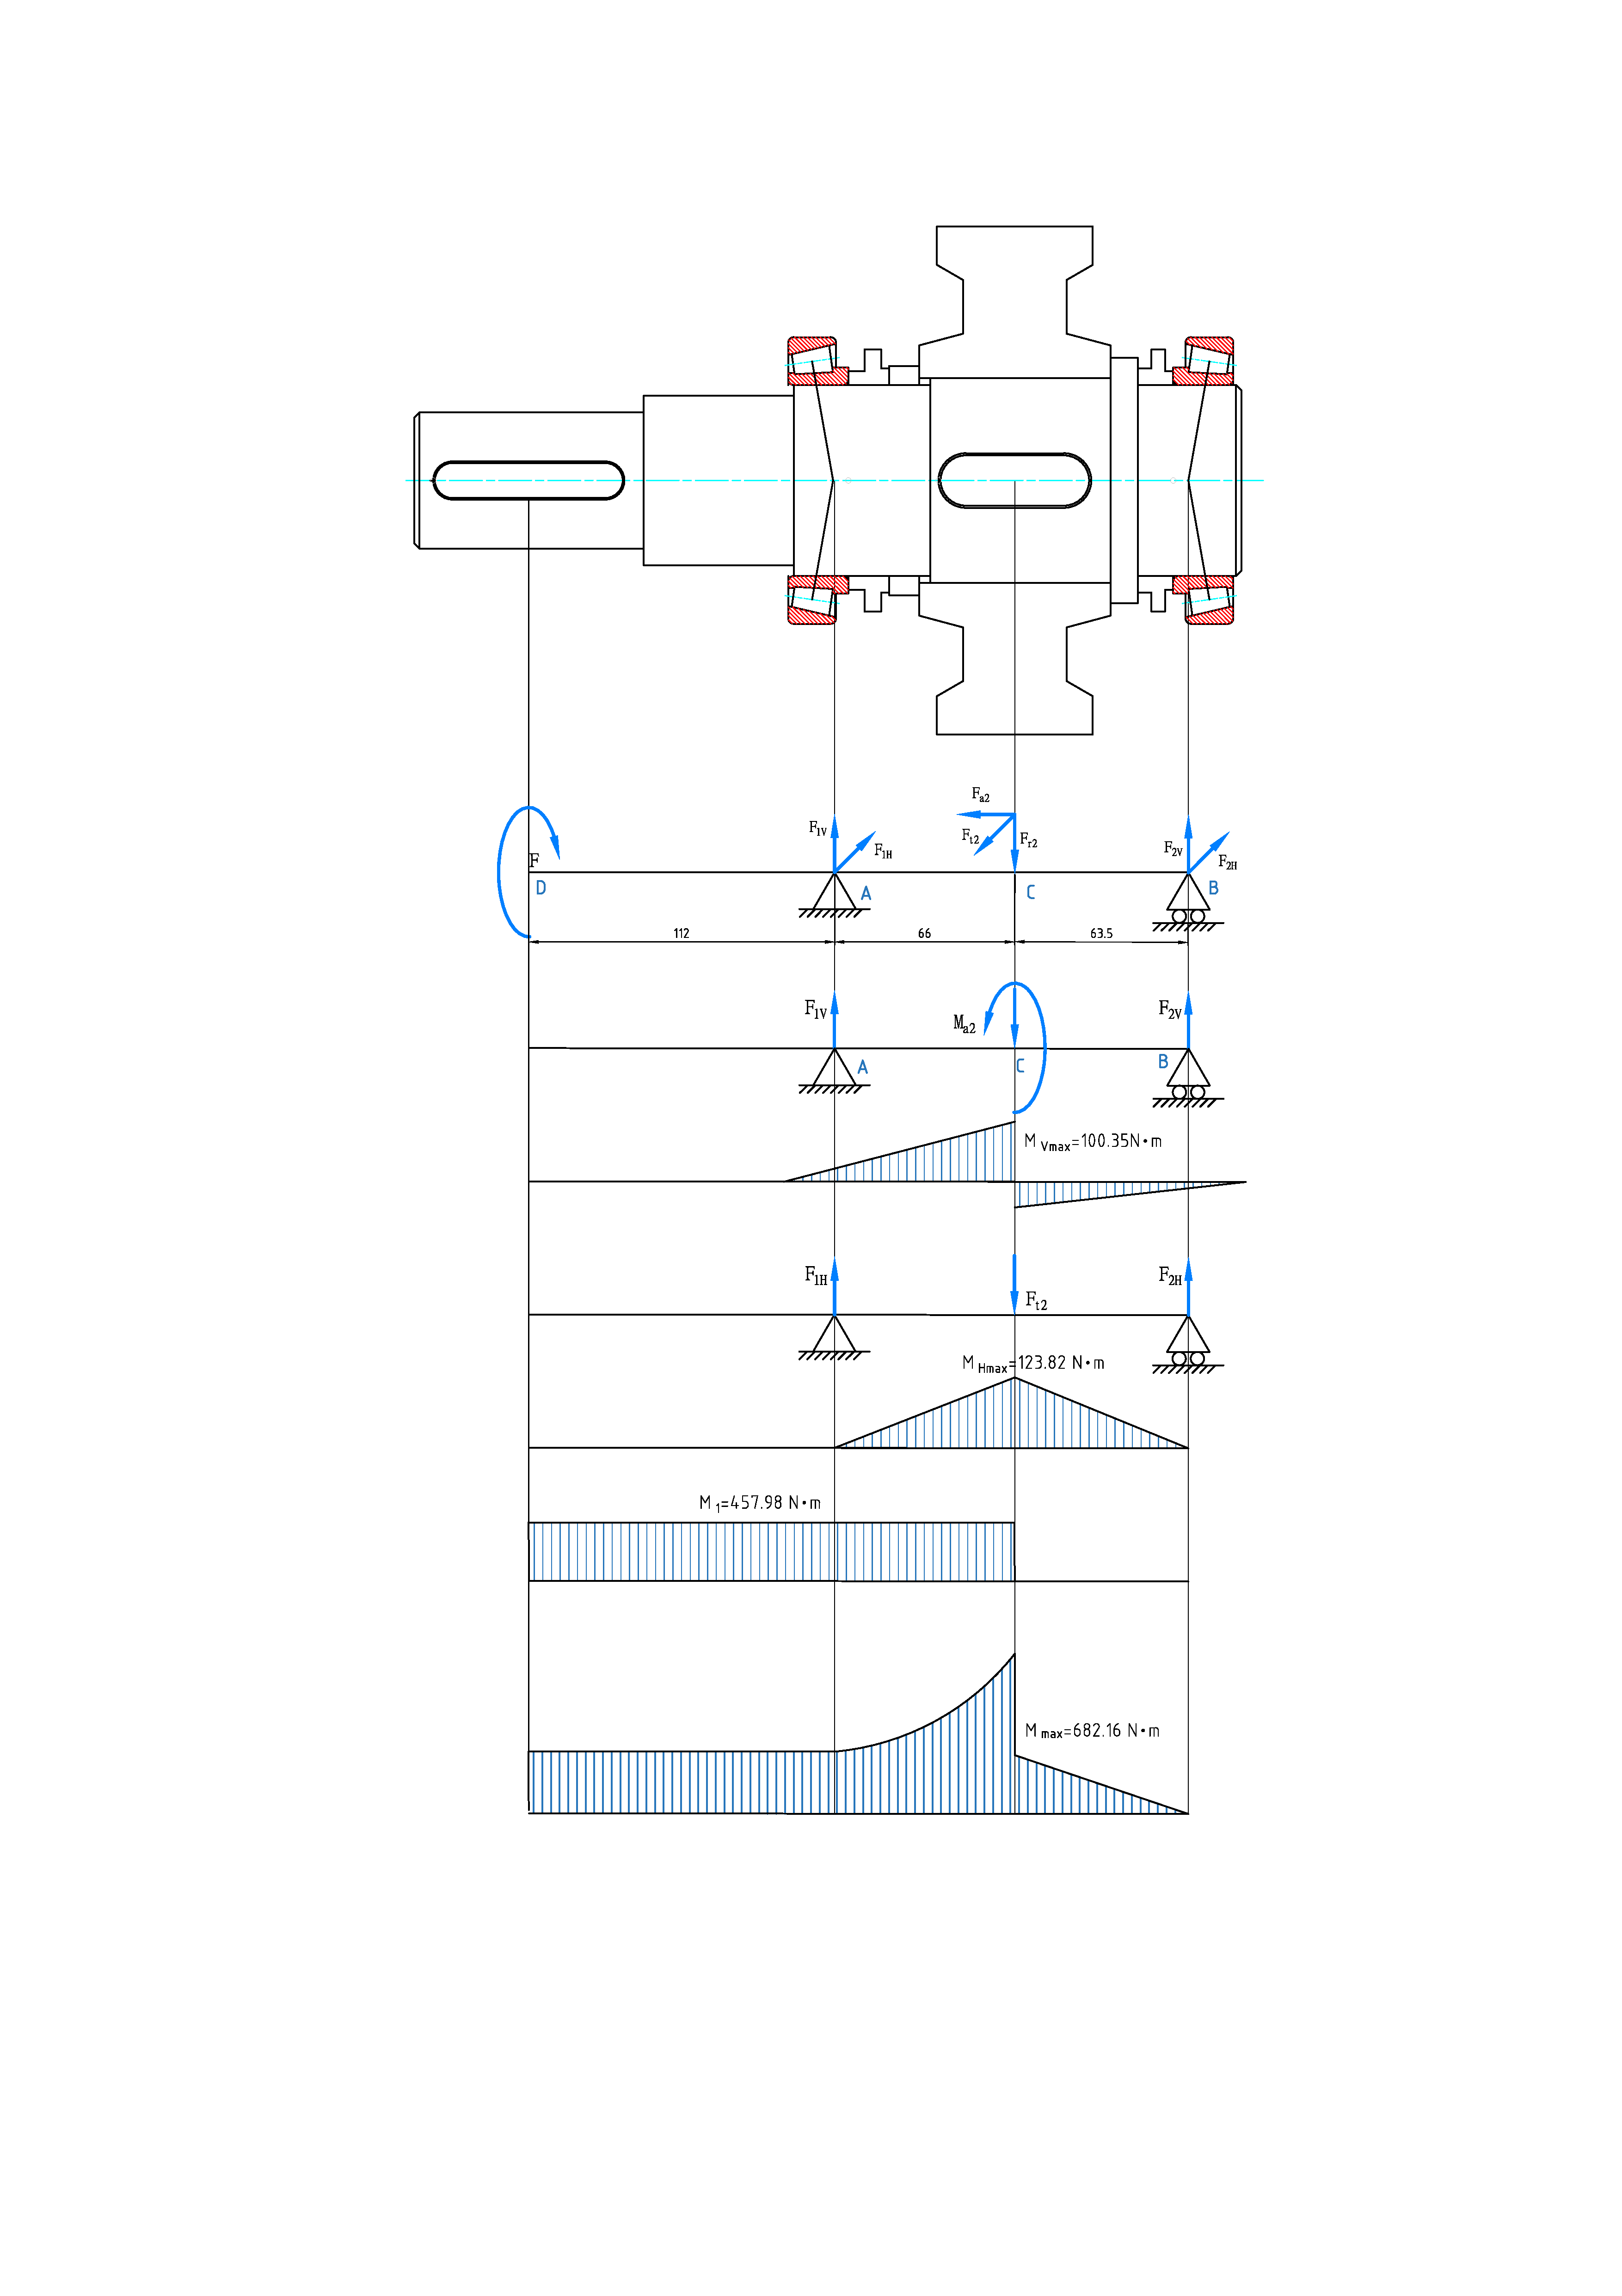
\includegraphics[width=0.8\linewidth]{蜗轮轴扭矩图}
		\caption{蜗轮轴扭矩图}
	\end{figure}
	
	\paragraph{3.危险截面强度校核}
	C截面的应力$\sigma_C=\frac{M_{max}}{0.1\cdot {d_2}^3}=7.11<[\sigma_F]=28\ Mpa$
	\paragraph{4.联轴器校核}
	此联轴器参数为:LT8$\ \frac{50 \times84}{60\times142}$GB/T\ 4323-2017,
	其\textbf{公称转矩为}:$T_n=1120 \ N\cdot m \ge T_{ca}=K_A T_1=1.3\times \two{\TII}=595.37\ N\cdot m$,满足要求。
	\paragraph{5.轴上零件的定位与连接方式}
	\begin{enumerate}
		\item[(1)] \ \ 联轴器与轴的定位采用A型平键%(两头是半圆)
		连接,参数为:GB/T\ 1096\  \ 键\ \ 18$\times$70,也采用完全对称偏差配合.\ \
		\item[(2)]轴承端盖通过轴承套筒定位,不与轴连接.
		\item[(3)]套筒通过凸台,轴肩定位,与轴采用间隙配合$\frac{H7}{h6}$   %都是基轴制
		\item[(4)]滚动轴承用轴肩定位,采用过盈配合$\frac{P7}{h6}$,
		\item[(5)]出轮轮毂与轴采用过盈配合$\frac{H7}{r6}$
	\end{enumerate}
	\paragraph{6.蜗轮轴(低速轴)键的校核}
	设载荷为均匀分布,可以计算得到该平键的挤压强度条件:
	\newcommand{\SiII}{\fpeval{4*457.98 /(18*10*70*0.01)}}
	$$\sigma_p=\frac{4T}{dhl}=\frac{4\cdot \two{\TII}\cdot 10^{2}}{18\cdot 10 \cdot 70}= \two{\SiII}\le [\sigma_p]=60\ MPa$$
	选取钢作为轮毂的材料,由以上计算可知,键的选取满足要求。
	\paragraph{7.轴承的校核}
	根据所选参数可知,蜗轮轴上的滚动轴承参数为:
		轴承选取$30214$ GB/T\ 297-2015,其参数为:$d\times D \times B=70\times125\times22$长度为$L_3=15+11+24=50\ mm$,其额定动载荷为$C_r=132000\ N$极限转速为3000,寿命取$10000h$	由受力分析易得右端为压紧端,查表可得$f_t\text{(温度系数)}=1,f_p\text{(载荷系数)}=1,\epsilon=\frac{3}{10}$由公式
	\begin{align*}
		C_r &= \frac{f_pP}{f_t}(\frac{60n}{10^6}L_h)^{\frac{1}{\epsilon}} \\
		132000 &= \frac{1\times P}{1}(\frac{60\times 50}{10^6}\times 10^4)^{\frac{3}{10}} \\
		P=F_r &= \frac{132000}{30^{0.3}}=4785> \two{\FtII}\ N
	\end{align*}
	所以轴承满足要求。
	
	
	\chapter{减速器箱体及附件的设计}
		根据计算的数据与经验,求得箱体的推荐尺寸如下:
	\begin{table}[h]\centering  %没有编程部分,等到以后有空再补上.-6-22
		%必须补了-6-24
		
		\begin{tabular}{c|c|c}
			\hline
			箱座壁厚               & $\delta=9.4\ mm$    & $0.04a+3\ge8\ mm$           \\ \hline
			箱盖壁厚               & $\delta_1=9.4\ mm$  & $ \approx \delta $          \\ \hline
			箱座凸缘厚度           & $b=14.1\ mm$        & $1.5\delta$                 \\ \hline
			箱盖凸缘厚度           & $b_1=14.1\ mm$      & $1.5\delta_1$               \\ \hline
			箱座底凸缘厚度         & $b_2=23.5\ mm$      & $2.5\delta$                 \\ \hline
			地脚螺栓直径           & $d_f=17.76\ mm$     & $0.036a+12$                 \\ \hline
			地脚螺栓数目           & $n=4\ mm$           & $4$                         \\ \hline
			轴承旁联接螺栓直径     & $d_1=13.32\ mm$     & $0.75d_f$                   \\ \hline
			箱盖与箱座联接螺栓直径 & $d_2=8.88\sim10.66$ & $(0.5\sim 0.6 d_f$          \\ \hline
			联接螺栓$d_2$的间距    & $l=175\ mm$         & $150\sim 200$               \\ \hline
			轴承端盖螺钉直径       & $d_3=7.10\sim8.88$  & $(0.4\sim 0.5) d_f$         \\ \hline
			窥视孔盖螺钉直径       & $d_4=5.32\sim7.10$  & $(0.3\sim 0.4) d_f$         \\ \hline
			定位销直径             & $d$                 & $(0.7\sim0.8) d_2$          \\ \hline
			轴承旁凸台半径         & $R_1$               & $c_2$                       \\ \hline
			凸台高度               & $h$                 & $根据d_1与与轴承座外径确定$ \\ \hline
			外箱壁到轴承座端面距离 & $l_1$               & $c_1+c_2(5\sim 8)$          \\ \hline
			蜗杆外圆与内壁距离     & $\Delta_1>11.28$    & $>1.2\delta$                \\ \hline
			蜗轮轮毂端面与内壁距离 & $\Delta_2>9.40$     & $>\delta$                   \\ \hline
			箱盖肋厚\dunhao 拉拉   & $m_1=7.99\ mm$      & $m_1\sim 0.85\delta_1$      \\ \hline
			箱座肋厚               & $m_2=7.99\ mm$      & $m_2\sim 0.85\delta$        \\ \hline
			轴承端盖外径           & $D_2$               & $4D+(5\sim 5.5)d_3$         \\ \hline
			轴承端盖凸缘厚度       & $t$                 & $(1\sim 1.2d_3)$            \\ \hline
			轴承旁联接螺栓距离     & $S$                 & $S\sim D_2$                 \\ \hline
		\end{tabular}
		\caption{箱体经验尺寸}
	\end{table}\ \
	\section{检查孔和视孔盖}
	{检查孔用于检查传动件的啮合情况、润滑状态、接触斑点及齿侧间隙,还可用来注入润滑油,故检查孔应开在便于观察传动件啮合区的位置,其尺寸大小应便于检查操作。}\par
	{	视孔盖可用铸铁、钢板制成,它和箱体之间应加密封垫,还可在孔口处加过滤装置,以过滤注入油中的杂质。参照表}
	
	\section{放油螺塞}
	{放油孔应设在箱座底面最低处或设在箱底。箱外应有足够的空间,以便于放容器,油孔下也可制出唇边,以利于引油流到容器内。放油螺塞常为六角头细牙螺纹,在六角头与放油孔的接触面处,应加封油圈密封。放油螺塞及对应油封圈尺寸如下图所示:}
	\begin{figure}[h!]
		\centering
		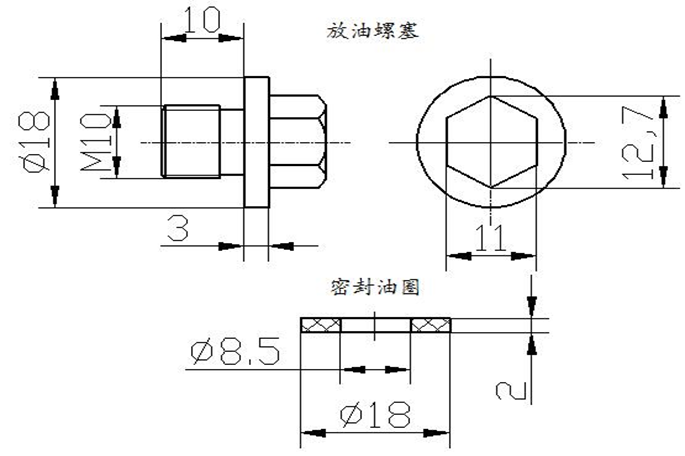
\includegraphics[width=0.7\linewidth]{photos/螺塞}
		\caption{放油螺塞}
		\label{fig:}
	\end{figure}
	
	
	\section{油标}
	{油标用来指示油面高度,应设置在便于检查及油面较稳定之处。本设计采用杆式油标,杆式油标结构简单,其上有刻线表示最高及最低油面。油标安置的位置不能太低,以防油溢出。其倾斜角度应便于油标座孔的加工及油标的装拆。查辅导书手册,具体结构和尺寸如下:}
	\begin{figure}[h!]
		\centering
		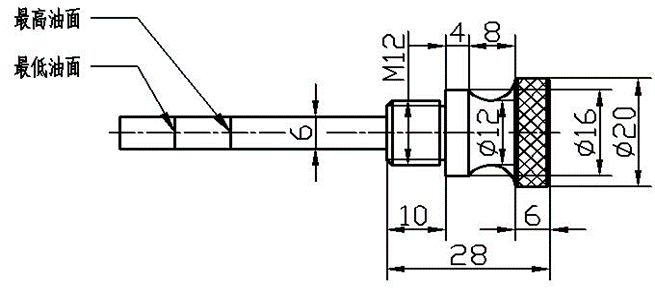
\includegraphics[width=0.7\linewidth]{photos/油标}
		\caption{油标}
		\label{fig:}
	\end{figure}
	
	
	\section{通气器}
	{通气器用于通气,使箱体内外气压一致,以避免由于运转时箱体内温度升高,内压增大,而引起减速器润滑油的渗漏。简易的通气器钻有丁字形孔,常设置在箱顶或检查孔盖上,用于较清洁的环境。较完善的通气器具有过滤网及通气曲路,可减少灰尘进入。查辅导书手册,本设计采用通气器型号及尺寸如下:}
	
	\section{起吊装置}
	{起吊装置用于拆卸及搬运减速器。它常由箱盖上的吊孔和箱座凸缘下面的吊耳构成。也可采用吊环螺钉拧入箱盖以吊小型减速器或吊起箱盖。本设计中所采用吊孔(或吊环)和吊耳的示例和尺寸如下图所示:}
	\begin{figure}[h!]
		\centering
		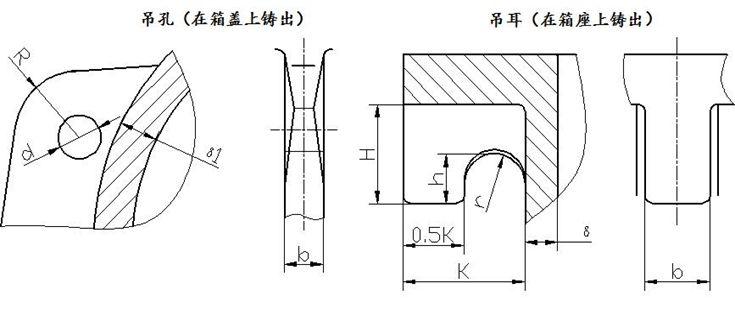
\includegraphics[width=0.7\linewidth]{photos/吊耳}
		\caption{吊耳}
		\label{fig:}
	\end{figure}
	
	
	\section{起盖螺钉}
	{为便于起箱盖,可在箱盖凸缘上装设2个起盖螺钉。拆卸箱盖时,可先拧动此螺钉顶起箱盖。
		起盖螺钉钉头部位应为圆柱形,以免损坏螺纹。本设计起盖螺钉尺寸如下:}
	
	\section{定位销}
	{保证箱体轴承孔的加工精度与装配精度,应在箱体连接凸缘上相距较远处安置两个圆锥销,并尽量放在不对称位置,以使箱座与箱盖能正确定位。
		为便于装拆,定位销长度应大于连接凸缘总厚度。本设计定位销尺寸如下:
	}
	\newpage
	\chapter*{设计小结}
	这次关于蜗轮蜗杆减速器(闭式齿轮传动)的课程设计是我们真正理论联系实际、深入了解设计概念和设计过程的实践考验,对于提高我们机械设计的综合素质大有用处。
	通过两个星期的设计实践,使我对机械设计有了更多的了解和认识,为我们以后的工作打下了坚实的基础.
	\begin{enumerate}
		\item 机械设计是机械工业的基础,是一门综合性相当强的技术课程,它融《机械原理》、《机械设计》、《理论力学》、《材料力学》、《公差与配合》、《CAD实用软件》、《机械工程材料》、《机械设计手册》等于一体。
		\item 这次的课程设计,对于培养我们理论联系实际的设计思想;训练综合运用机械设计和有关先修课程的理论,结合生产实际关系和解决工程实际问题的能力;巩固、加深和扩展有关机械设计方面的知识等方面有重要的作用。
		\item 在这次的课程设计过程中,综合运用先修课程中所学的有关知识与技能,结合各个教学实线环节进行机械课程的设计,一方面,逐步提高了我们的理论水平、构思能力、工程洞察力和判断力,特别是提高了分析问题和解决问题的能力,为我们以后对专业产品和设备的设计打下了宽广而坚实的基础
		\item 设计中还存在不少错误和缺点,需要继续努力学习和掌握有关机械设计的知识,继续培养设计习惯和思维从而提高设计实践操作能力
		
		\item 本次设计得到了指导老师的细心帮助和支持。衷心的感谢老师的指导和帮助.
		 
	\end{enumerate}
	\begin{thebibliography}{66}
		
		\bibitem[1]{电动机}  《GB/T 28575-2012 YE3系列(IP55)超高效率三相异步电动机技术条件》
		\bibitem[2]{课本} 濮良贵、陈国定、吴立言.《机械设计第9版》.北京,高等教育出版社,
		\bibitem[3]{1}龚桂义.机械设计课程设计图册
		\bibitem[4]{2}王之栎, 王大康. 机械设计综合课程设计[M]. 机械工业出版社, 2009.
		\bibitem[5]{5}陈云飞 卢玉明. 机械设计基础(第7版)[M]. 高等教育出版社, 2008.
		\bibitem[6]{citekey}同济大学、上海交通大学等院校《机械制图》编写组. 机械制图.第6版[M]. 高等教育出版社, 2010.
		
		
		\addcontentsline{toc}{chapter}{参考文献}
	\end{thebibliography}
\end{document}